%%%%%%%%%%%%%%%%%%%%%%%%%%%%%%%%%%%%%%%%%%%%%%%%%%%%%%%%%%%%%%%%%%%%%%%%%%%
%% Bachelor's & Master's Thesis Template                                 %%
%% Copyleft by Dawid Weiss & Marta Szachniuk                             %%
%% Faculty of Automatic Control, Robotics, and Electrical Engineering    %%
%% Poznan University of Technology, 2023                                 %%
%%%%%%%%%%%%%%%%%%%%%%%%%%%%%%%%%%%%%%%%%%%%%%%%%%%%%%%%%%%%%%%%%%%%%%%%%%%


% Szkielet dla pracy inżynierskiej/magisterskiej pisanej w języku polskim.
\documentclass[polish,bachelor,a4paper,oneside]{ppcreefthesis}

% Template for an engineering/master's thesis written in English.
% \documentclass[english,bachelor,a4paper,oneside]{ppcreefthesis}


\usepackage[utf8]{inputenc}
\usepackage[OT4]{fontenc}
\usepackage{xcolor}   % Do kolorowania tekstu
\usepackage{soul}      % Do podkreślania i podświetlania tekstu
\usepackage[usenames,dvipsnames]{xcolor}
\usepackage{graphicx}
\usepackage{tabularx}
\usepackage{multirow}
\usepackage{multicol}
\usepackage{array}
\usepackage{float}
\usepackage{changepage}
\usepackage{tikz}
\usetikzlibrary{shapes, arrows, positioning,shapes.geometric, calc}
\usepackage{adjustbox}
\usepackage{hyperref}
\usepackage{subcaption}
\usepackage{enumitem}
\usepackage{listings}
\usepackage{enumitem}
\usepackage{longtable}

\newcommand{\customnote}[1]{\sethlcolor{yellow}\hl{#1}}



\newcolumntype{W}{>{\centering\arraybackslash}p{5cm}}
\newcolumntype{w}{>{\centering\arraybackslash}m{1.2cm}}


%--------------------------------------
% Strona tytułowa \ Front page
%--------------------------------------

% Autorzy pracy, jeśli jest ich więcej niż jeden
% wstaw między nimi separator \and

% Authors of the thesis, if there is more than one
% insert a separator between them \and

\author{%
   Remigiusz Wolniak \album{151192} \and 
   Michał Gajdzis \album{151066} }
\authortitle{}                                % Do not change.

\title{Automatyzacja procesu planowania wydatków na~usługi IT w VW Poznań z wykorzystaniem Microsoft~Power~Platform}

% Promotor pracy
% Your supervisor comes here.

\ppsupervisor{dr hab.~inż.~Piotr~Kaczmarek} 
\ppinstitute{Instytut Robotyki i Inteligencji Maszynowej \\ }
 %            Zakład Sterowania i Elektroniki Przemysłowej

% Rok złożenia pracy
% Year of final submission (not graduation!)
\ppyear{2025}                                 


\begin{document}

% Pierwsza strona zaczyna się tutaj



% Front matter starts here
\frontmatter\pagestyle{empty}%
\maketitle\cleardoublepage%

% Ponizej tresc na pierwsza strone pracy dyplomowej z VW (od Kroteckiego)

\begin{center}
    \Large \textbf{Zastrzeżenie dotyczące treści pracy dyplomowej}
\end{center}

\vspace{1cm}

%\onehalfspacing % Ustawienie interlinii 1.5

Niniejsza praca inżynierska zawiera treści, informacje itp. udostępnione przez spółkę Volkswagen Poznań Sp.
z o.o.
z siedzibą przy ulicy Warszawskiej 349, 61-060 w Poznaniu, mogące stanowić
tajemnice przedsiębiorstwa tej spółki i mogące być wykorzystane wyłącznie dla
potrzeb napisania niniejszej pracy. Wobec powyższego niedozwolone jest
wykorzystywanie całości lub części niniejszej pracy, a także udostępnianie całości
lub części pracy komukolwiek jak również kopiowanie, powielanie, publikowanie itp.
bez pisemnej zgody spółki Volkswagen Poznań Sp. z o.o. -- zastrzeżenie to nie ma
zastosowania do przypadku udostępnienia niniejszej pracy nauczycielom
akademickim w celu oceny, recenzji
i obrony ww. pracy. Podmioty, które naruszą powyższy zakaz ponoszą
odpowiedzialność odszkodowawczą wobec spółki Volkswagen Poznań Sp. z o.o.

%--------------------------------------
% Miejsce na kartę pracy dyplomowej - opcjonalnie, nie jest wymagane
%--------------------------------------
\thispagestyle{empty}\vspace*{\fill}%
\begin{center}Tutaj będzie skan karty pracy dyplomowej. \end{center}%
\vfill\cleardoublepage%
%--------------------------------------


%--------------------------------------
% Spis treści
%--------------------------------------

\pagenumbering{Roman}
\pagestyle{ppfcmthesis}
\tableofcontents*
\cleardoublepage % Zaczynamy od nieparzystej strony

%--------------------------------------
% Rozdziały
%--------------------------------------

%Najwygodniej jeśli każdy rozdział znajduje się w oddzielnym pliku
\mainmatter%
\chapter{Wstęp}

    \textcolor{red}{Współczesny świat biznesu stawia coraz większe wymagania wobec przedsiębiorstw, zarówno w zakresie efektywności procesów, jak i precyzji podejmowanych działań. Proces ten, dotychczas realizowany manualnie z wykorzystaniem tradycyjnych narzędzi do zarządzania danymi, wiązał się z dużym nakładem pracy, czasochłonnością, a także znacznym ryzykiem błędów ludzkich. W obliczu tych wyzwań coraz większą rolę odgrywają rozwiązania z zakresu automatyzacji biurowej, które umożliwiają usprawnienie kluczowych procesów organizacyjnych, minimalizując ryzyko błędów ludzkich oraz oszczędzając czas i zasoby.} \par Jednym z najważniejszych obszarów, w którym automatyzacja znajduje zastosowanie, jest zarządzanie usługami IT i powiązanymi kosztami. W dużych organizacjach, takich jak korporacje o rozbudowanej strukturze, konieczność zbierania, analizy oraz weryfikacji danych finansowych związanych z usługami IT stanowi poważne wyzwanie. Dzięki wdrożeniu odpowiednich narzędzi, procesy te mogą być prowadzone w sposób bardziej przejrzysty, zorganizowany i efektywny, umożliwiając jednocześnie bieżącą kontrolę nad wydatkami oraz lepsze planowanie budżetowe. \par{
    Ustandaryzowany i zautomatyzowany przepływ informacji ogranicza ryzyko powielania błędów i pozwala na skrócenie czasu potrzebnego na wykonanie poszczególnych etapów procesów. Co więcej, wdrożenie automatyzacji zapewnia większą przejrzystość i umożliwia każdemu uczestnikowi procesu łatwy dostęp do potrzebnych informacji w odpowiednim czasie. \par W dobie intensywnej cyfryzacji przedsiębiorstw oraz dynamicznego rozwoju technologii, automatyzacja biurowa staje się nie tylko opcją, ale wręcz koniecznością, aby sprostać wymaganiom współczesnego rynku. Odpowiednio zaprojektowane systemy i narzędzia wspierają nie tylko wydajność operacyjną, ale także strategiczne zarządzanie zasobami, umożliwiając organizacjom rozwój i utrzymanie konkurencyjności.}



\chapter{Wstęp szablon}

Wstęp do pracy powinien zawierać następujące elementy:
\begin{itemize}
    \item krótkie uzasadnienie podjęcia tematu; 
    \item cel pracy (patrz niżej); 
    \item zakres (przedmiotowy, podmiotowy, czasowy) wyjaśniający, w jakim rozmiarze praca będzie realizowana; 
    \item ewentualne hipotezy, które autor zamierza sprawdzić lub udowodnić; 
    \item krótką charakterystykę źródeł, zwłaszcza literaturowych; 
    \item układ pracy (patrz niżej), czyli zwięzłą charakterystykę zawartości poszczególnych rozdziałów; 
    \item ewentualne uwagi dotyczące realizacji tematu pracy np.~trudności, które pojawiły się w trakcie 
    realizacji poszczególnych zadań, uwagi dotyczące wykorzystywanego sprzętu, współpraca z firmami zewnętrznymi. 
\end{itemize}

\noindent
\textbf{Wstęp do pracy musi się kończyć dwoma następującymi akapitami:}
\begin{quote}
Celem pracy jest opracowanie / wykonanie analizy / zaprojektowanie / ...........
\end{quote}
oraz:
\begin{quote}
Struktura pracy jest następująca. W rozdziale 2 przedstawiono przegląd literatury na temat ........ 
Rozdział 3 jest poświęcony ....... (kilka zdań). 
Rozdział 4 zawiera ..... (kilka zdań) ............ itd. 
Rozdział X stanowi podsumowanie pracy. 
\end{quote}

W przypadku prac inżynierskich zespołowych lub magisterskich 2-osobowych, po tych dwóch w/w akapitach 
musi w pracy znaleźć się akapit, w którym będzie opisany udział w pracy poszczególnych członków zespołu. Na przykład:

\begin{quote}
Jan Kowalski w ramach niniejszej pracy wykonał projekt tego i tego, opracował ......
Grzegorz Brzęczyszczykiewicz wykonał ......, itd. 
\end{quote}



\chapter{Podstawy teoretyczne}

%\newline\textcolor{orange}{
%Można coś dopisać/ poprawić to powyżej. Chciałem tutaj przedstawić zarys jak wygląda proces.
%myśle żeby poniżej w każdym akapicie opisać krok po kroku jak to wyglądało z użyciem exceli.
%Tylko trzeba to napisać sensownie i łądnie żeby nikt się nie zajebał w akcji i żeby uwzględnić
%wszystkie rzeczy. Tutaj chyba nie będziemy się rozwodzili na temat minusów tego rozwiązania.
%no i potem bym dał informacje na temat użytych technologii: typescript, sharepoint, power au-
%tomate i power apps. imo taka kolejność żeby odzwierciedlała trochę jaki jest proces w apce bo
%bedziesz mógł się odwołąć do poprzednich. np że automate zaciaga dane z SP i każdy wie czym
%jest już sharepoint i essa.}
\section{Struktura procesu}
% Przedmiotem omawianego procesu jest podjęcie decyzji na tematu zakupu usług IT w zakładzie
% Volkswagen Poznań. Polega on na wymianie uwag, dotyczących wcześniej używanego bądź nowego
% oprogramowania, między oddziałem Volkswagen w Poznaniu a zakładem z siedzibą w Wolfsburgu.
Przedmiotem omawianego procesu jest podjęcie decyzji dotyczących zakupu usług IT w zakładzie Volkswagen Poznań. Proces ten polega na wielokrotnej wymianie uwag dotyczących wcześniej używanego lub nowego oprogramowania między oddziałem Volkswagena w Poznaniu a zakładem z siedzibą w Wolfsburgu.

W wyniku wymiany zdań zapada decyzja o zakupie lub rezygnacji z wybranego produktu. Procedura, zazwyczaj podzielona na cztery {indykacje}\footnote{\emph{indykacja}  - wstępne głosowanie}, rozpoczyna się wraz z początkiem czerwca i trwa do końca roku.

Efektem podejmowanych działań jest nabycie odpowiedniej ilości potrzebnych uprawnień licencyjnych. Przy
podejmowaniu decyzji kluczowymi aspektami są:
\begin{itemize}
    \item liczba użytkowników danego oprogramowania,
    \item cena zakupu w porównaniu z rokiem poprzednim,
    \item określenie, czy dana usługa zostanie w pełni wykorzystana biorąc pod uwagę poprzednie kryteria.
\end{itemize}
Dotychczas analiza i przetwarzanie danych odbywały się przy użyciu arkuszy kalkulacyjnych programu Excel, a wymiana informacji między jednostkami była realizowana za pomocą wiadomości e-mail.
\subsection{Gromadzenie danych dotyczących ofert usługodawców}
Informacje na temat serwisów są zbierane na początku roku, przed rozpoczęciem cyklu procesu. W tym czasie, prowadzone są rozmowy między menadżerami odpowiedzialnymi za dane rozwiązanie (\akronim{BSM}, \english{Business Service Manager}) a firmami świadczącymi usługi, w celu otrzymania zaaktualizowanych wiadomości związanych z ich produktami. Na podstawie danych od usługodawców oraz menadżerów, powstaje arkusz, który jest przekazywany do zakładu w Poznaniu.
\subsection{Przygotowanie danych}
Otrzymany arkusz kalkulacyjny, zawiera tabelę o strzukturze kolumn podobnej do tabeli \ref{Headers2022}. Brakuje w nim jednak informacji kluczowych do rozpoczęcia cyklu.
Dlatego pierwszym krokiem jest przygotowanie danych przez osobę nadzorującą proces ze strony odziału w Poznaniu.
Jej zadaniem jest manualne przypisanie numeru określającego miejsce powstawania kosztów, wewnętrznie nazywanego \definicja{MPK}. Numer ten definiuje konkretną jednostkę należącą do obszaru IT, która decyduje o zakupie danego produktu. Ponadto, dodawana jest kolumna, w której znajduje się wyliczona różnica cen między rokiem obecnym a poprzednim, w celu określenia czy koszt wzrósł lub zmalał. Tak przetworzony plik zostaje umieszczony we wspólnej przestrzeni dyskowej, co umożliwia pozostałym uczestnikom procesu przystąpienie do analizy oraz dalszego przetwarzania zawartych w nim informacji.

\renewcommand{\arraystretch}{1.1} % Zwiększenie wysokości komórek
\begin{table}[H] % [H] - tabela dokładnie w tym miejscu
    \begin{adjustwidth}{-50pt}{-20pt}
        \centering
        \caption{Nagłówki kolumn z arkusza kalkulacyjnego z roku 2022}
        \label{Headers2022}
        \makebox[\textwidth][c]{%
            \begin{tabular}{*{3}{|m{1.1cm}}|w|m{0.4cm}|m{1.5cm}|m{1.75cm}|w|m{0.7cm}|w|m{0.7cm}|}
                \hline
                Service group & Service main group & Service sub group & Business Service & ID & Business Service Manager & Unit of Measurement & PL70 2022 PLAN EUR w KVA & QTY & PL71 2023 PLAN EUR w KVA & QTY \\ \hline
            \end{tabular}
        }
    \end{adjustwidth}
\end{table}

\subsection{Przebieg Iteracji}
W trakcie trwania iteracji analizowane są kluczowe informacje, takie jak:
\begin{itemize}
    \item jednostka miary (ang. \emph{Unit of Measurement}),
    \item decyzja podjęta w roku poprzednim,
    \item cena oraz liczba użytkowników w roku obecnym,
    \item cena oraz liczba użytkowników w roku przyszłym.
\end{itemize}
Po analizie i porównaniu danych z wcześniejszych lat, w arkuszu powstają kolejne kolumny. Ich struktura nie jest określona przez żaden standard, ale zazwyczaj zawierają one:
\begin{itemize}
    \item Komentarz wewnętrzny,
    \item Status,
    \item Komentarz klienta.
\end{itemize}

\noindent\emph{Komentarz wewnętrzny} nie jest wymagany dla każdego serwisu. Jest on zapisywany w celu skonsultowania decyzji ze współpracownikami.\\ \emph{Status} określa wstępną, wymaganą decyzję (Zaakceptowany/Niezaakceptowany).\\ \emph{Komentarz klienta} zawiera uzasadnienie podjętej decyzji ze strony Volkswagen Poznań.\\Tak uzupełniony arkusz zostaje przekazany pośrednio przez zakład w Wolfsburgu do zarządu firmy. \par
Kolejnym etapem jest analiza tych informacji przez wcześniej wymienione podmioty. Ich zadaniem jest konfrontacja podjętej decyzji. Dodawane są kolejne kolumny:
\begin{itemize}
    \item Komentarz BSM,
    \item Komentarz K-DES.
\end{itemize}

\noindent\emph{Komentarz BSM} to opinia wyrażona przez menedżera usługi, natomiast \emph{Komentarz K-DES} stanowi odpowiedź międzynarodowego zarządu firmy, który odpowiada za kształtowanie strategii IT.\par
Zaaktualizowany plik powraca do Volkswagen Poznań, rozpoczynając tym samym kolejną iterację procesu.







% Podsumowanie przebiegu proceso - nie tworzyłem nowego pliku na dwa zdania.
\vspace{1cm}
Jak wcześniej wspomniano, proces składa się zazwyczaj z czterech iteracji. Etapem kończącym cykl jest sporządzenie wymaganych dokumentów oraz faktur.

\section{Wykorzystane technologie}
Aby usprawnić przebieg procesu, zabiezpieczyć go przed błędami i usystematyzować, stworzona została aplikacja do jego obsługi. Głównym kryterium przy doborze technologii była powszechna dostępność do powstałego systemu wśród pracowników. Dlatego też zdecydowano się na wykorzystanie komponentów pakietu \emph{Office 365}. Pakiet ten jest bardzo rozbudowany i jest powszechnie używany w firmie Volkswagen. Zawiera on programy pozwalające na stworzenie kompletnego systemu bez konieczności dostępu do dodatkowych usług.
\subsection{Skrypty pakietu Office}
Skrypty pakietu Office pozwalają na automatyzacje zadań w arkuszach kalkulacyjnych Excel. Jedną z dostępnych opcji jest  funkcja \emph{Action Recorder}, która daje możliwość "nagrania" sekwencji kroków wykonanych przez użytkownika, a następnie przekształca je na skrypt wielokrotnego użytku.\par
Skrypty pakietu Office dysponują również wbudowanym \emph{edytorem kodu} (\english{Code Editor}), opartym na języku \emph{TypeScript}, będącym odmianą \emph{JavaScript}. Sam edytor, choć stosunkowo ograniczony, umożliwia zastosowanie konstrukcji niedostępnych w Action Recorder, takich jak instrukcje warunkowe czy pętle.\par
Ponadto program Excel pozwala na zapis skryptu w skoroszycie. Oznacza to, że każdy użytkownik dysponujący dostępem do pliku uzyskuje również możliwość uruchomienia kodu powiązanego ze skoroszytem, do którego jest on przypisany.
\subsection{SharePoint}
SharePoint to platforma wchodząca w skład pakietu Microsoft 365, która służy do zarządzania dokumentami oraz umożliwia efektywną współpracę zespołową. Dzięki niej użytkownicy mogą tworzyć i korzystać z własnych przestrzeni roboczych online, takich jak listy czy archiwa plików, co znacząco ułatwia organizację oraz szybki dostęp do danych.

Listy sharepointowe mogą pełnić funkcję prostych baz danych, które można łatwo zintegrować z takimi narzędziami jak PowerApps, PowerAutomate, czy Excel. Takie rozwiązanie umożliwia dynamiczne aktualizowanie i synchronizowanie danych w czasie rzeczywistym.



\subsection{Power Automate }
Power Automate to narzędzie wchodzące w skład pakietu Microsoft 365, które umożliwia automatyzację procesów biznesowych (\akronim{RPA}, \english{Robotic Process Automation}). Pozwala ono na~tworzenie przepływów pracy (\english{flows}), automatyzujących powtarzalne zadania i integrujących różne systemy, zwiększając efektywność procesów biznesowych.

Flow w Power Automate jest odpowiednikiem funkcji w standardowych językach programowania. Na przykład przepływ może automatycznie wysyłać powiadomienia e-mail po aktualizacji rekordu w SharePoint. Różnica polega na tym, że jest on tworzony w wizualnym środowisku Low-Code i~działa na zasadzie logicznego ciągu akcji wyzwalanych kolejno przez określone instrukcje.

Za pomocą flow można tworzyć własne procesy, które przy odpowiedniej implementacji, dorównują tym znanym z pełnych środowisk kodowych pod względem logiki i efektywności. Do dyspozycji są instrukcje warunkowe, pętle, zmienne, operacje na danych czy integracje z API poprzez konektory \texorpdfstring{\cite{v-aangie_official_nodate}}{}.

\subsection{Power Apps}

Power Apps to środowisko Low-Code'owe, wchodzące w skład pakietu Office 365, które jest dedykowanym rozwiązaniem do tworzenia aplikacji biznesowych. Dzięki intuicyjnemu interfejsowi graficznemu daje możliwość prostej implementacji mechanizmu działania nawet przez osoby bez zaawansowanej wiedzy programistycznej. Jest ona zintegrowana z innymi usługami pakietu Office 365, takimi jak SharePoint czy Power Automate, co rozszerza możliwości stworzonych aplikacji.

Power Apps pozwala na stworzenie spersonalizowanej aplikacji, dostosowanej do motywu organizacji, a przy połączeniu z innymi serwisami daje możliwość tworzenia zaawansowanych rozwiązań, minimalizując przy tym czas potrzebny na ich zaimplementowanie.

Ekrany aplikacji, komponowane za pomocą tego rozwiązania, porównywalne są z tymi, które można stworzyć w standardowych środowiskach programistycznych (jak np. JavaScript czy .NET), jednak proces ich tworzenia jest prostszy, ze względu na obecność edytora wizualnego. Umożliwia on korzystanie z gotowych komponentów w aplikacji, takich jak przyciski, pola danych wejściowych, listy, tabele, grafiki etc.

Dodawanie elementów do ekranów aplikacji odbywa się poprzez przeciąganie ich z biblioteki i upuszczanie w wybranym miejscu. Każdy komponent, może zostać skonfigurowany według potrzeb użytkownika poprzez edycje \emph{właściwości}. Możemy określić między innymi wypełnienie czy pozycję \emph{X} i \emph{Y} na ekranie, ale niektóre obiekty mają też unikalne właściwości takie jak \emph{OnSelect} \footnote{OnSelect -- określa akcje, które zostaną wykonane po naciścięciu elementu} dla przycisku.


\newpage

\begin{figure}[h] % h - tu, t - góra, b - dół, p - strona dodatkowa
    \centering
    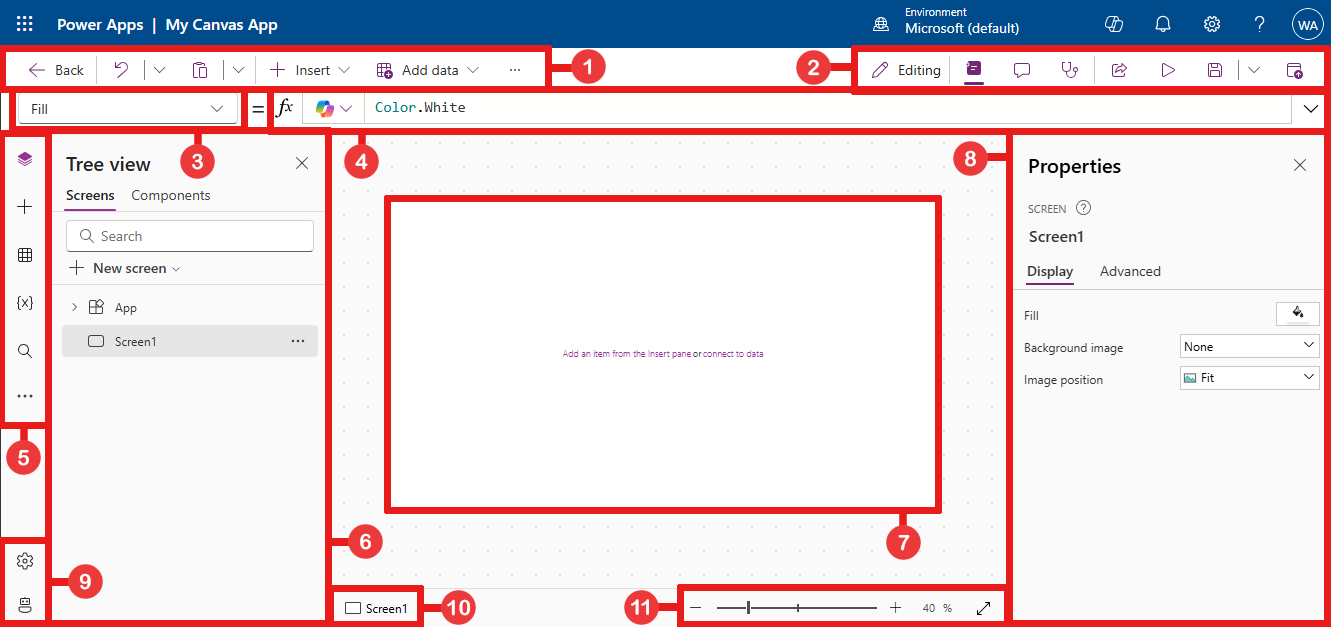
\includegraphics[width=\textwidth]{figures/PowerAppsOverview}
    \caption{Edytor Power Apps}
    \label{fig:PowerAppsEditorOverview}
\end{figure}
\textcolor{red}{LINK DO OBRAZKA I OPISU ELEMENTÓW: https://learn.microsoft.com/en-us/power-apps/maker/canvas-apps/power-apps-studio}

Rysunek \ref{fig:PowerAppsEditorOverview} przedstawia edytor programu. Zawiera on następujące elementy:
\begin{enumerate}
    \item \textbf{Pasek poleceń:} wyświetla inny zestaw poleceń w zależności od wybranego kontrolki.
    \item \textbf{Akcje aplikacji:} Opcje wyświetlania właściwości, dodawania komentarzy, sprawdzania błędów, udostępniania, podglądu, zapisu lub publikowania aplikacji.
    \item \textbf{Lista właściwości:} Lista właściwości wybranego obiektu.
    \item \textbf{Pasek formuł:} Tworzenie lub edycja formuły dla wybranej właściwości z użyciem jednej lub więcej funkcji.
    \item \textbf{Menu tworzenia aplikacji:} Panel wyboru umożliwiający przełączanie się między źródłami danych oraz wstawianie dodatkowych opcji.
    \item \textbf{Lista elementów aplikacji:} Pokazuje lementy obecne na ekranie w postaci drzewa.
    \item \textbf{Płótno/ekran:} Główne płótno do komponowania struktury aplikacji.
    \item \textbf{Panel właściwości:} Lista właściwości wybranego obiektu.
    \item \textbf{Ustawienia i wirtualny agent:} Ustawienia aplikacji lub uzyskanie pomocy od wirtualnego agenta.
    \item \textbf{Selektor ekranu:} Przełączanie się między różnymi ekranami w aplikacji.
    \item \textbf{Zmiana rozmiaru płótna:} Zmienianie rozmiaru wyświetlanego płótna podczas tworzenia aplikacji.
\end{enumerate}


















\chapter{Architektura rozwiązania}

Niniejszy rozdział przedstawia architekturę rozwiązania, obejmującą zarówno założenia projektowe, jak i koncepcję opracowywanego systemu. Założenia projektowe określają podstawowe wymagania oraz wytyczne, stanowiąc fundament opracowywanego rozwiązania. Natomiast koncepcja rozwiązania, uwzględniająca zasadnicze założenia, strukturę i logikę działania, stanowiące podstawę do dalszego prowadzenia prac projektowych.

\section{Założenia projektowe}
Założenia projektowe definiują podstawowe wytyczne dotyczące funkcjonalności i wymagań technicznych tworzonego rozwiązania. Obejmują one m.in. systematyzację danych, wykorzystanie platformy Microsoft 365 oraz optymalizację procesów decyzyjnych.




\subsection{Systematyzacja danych}
Jedną z zasadniczych funkcji omawianej aplikacji jest systematyzacja danych. Arkusze kalkulacyjne przesyłane przez oddział w Wolfsburgu nie posiadają ustandaryzowanej struktury, co negatywnie wpływa na ich czytelność oraz czas potrzebny na analizę.

\noindent Tabela \ref{HeaderComparison} przedstawia różnice w nazwach kolumn na przestrzeni trzech lat.

\renewcommand{\arraystretch}{1.3} % Zwiększenie wysokości komórek
\begin{table}[H] % [t] - tabela bliżej górnej krawędzi strony
   \centering
   \caption{Zestawienie nagłówków kolumn w latach 2022-2024}
   \label{HeaderComparison}
   \makebox[0.925\textwidth][c]{%
      \begin{tabular}{|c|W|W|W|}
         \hline
          & \textbf{2022}            & \textbf{2023}            & \textbf{2024}            \\ \hline
         \multirow{12}{*}{\rotatebox{90}{\parbox{3cm}{\centering \textbf{Nazwy kolumn na   \\przestrzeni lat}}}}
          & Service group            & Service group            & Service group            \\ \cline{2-4}
          & Service main group       & Service main group       & Service main group       \\ \cline{2-4}
          & Service sub group        & Service sub group        & Service sub group        \\ \cline{2-4}
          & Business Service         & Business Service         & Business Service         \\ \cline{2-4}
          & ID                       & ID                       & ID                       \\ \cline{2-4}
          & Business Service Manager & Business Service Manager & Business Service Manager \\ \cline{2-4}
          & Unit of Measurement      & Unit of Measurement      & Resource Unit            \\ \cline{2-4}
          &                          & Settlementtype           & Settlementtype           \\ \cline{2-4}
          & PL70 2022 PLAN EUR w KVA & PL71 2023 PLAN EUR w KVA & PL72 2024 PLAN EUR w KVA \\ \cline{2-4}
          & QTY                      & QTY                      & QTY                      \\ \cline{2-4}
          & PL71 2023 PLAN EUR w KVA & PL72 2024 PLAN EUR w KVA & PL73 2025 PLAN EUR w KVA \\ \cline{2-4}
          & QTY                      & QTY                      & QTY                      \\ \hline
      \end{tabular}
   }
\end{table}

Brak jednolitego formatu danych uniemożliwia również stworzenie spójnej bazy, co ogranicza możliwość ich wykorzystania w systemach automatyzacji procesów biznesowych. Dzięki wdrożeniu omawianego rozwiązania możliwe jest ujednolicenie danych, co pozwala na efektywne nimi zarządzanie i automatyczne przetwarzanie.
\subsection{Archiwizacja danych}
Utworzenie bazy danych gromadzącej informacje o wcześniejszych działaniach realizowanych w ramach projektowanego systemu stanowi istotny element zapewniający ciągłość procesów decyzyjnych. Dzięki systematycznej archiwizacji nowi użytkownicy mogą szybko zapoznać się z przebiegiem procedur i lepiej zrozumieć kontekst dotychczas podejmowanych decyzji. Dostęp do zasobów historycznych nie tylko skraca czas potrzebny na pełne wdrożenie w funkcjonowanie systemu, lecz także usprawnia przetwarzanie danych bieżących.
\subsection{Interfejs przyjazny dla użytkownika}
\begin{comment}Dedykowane narzędzie z prostym i intuicyjnym interfejsem znacząco ułatwia nawigację po bazie danych, eliminując problemy związane z tradycyjnymi rozwiązaniami, takimi jak arkusze kalkulacyjne. \end{comment}

Dzięki dedykowanemu narzędziu z prostym i intuicyjnym interfejsem, nawigacja po bazie danych jest znacznie prostsza, a problemy związane z używaniem arkuszy kalkulacyjnych zostają wyeliminowane. Przyjazny dla użytkownika interfejs oznacza:
\begin{itemize}
    \item \textbf{Prostotę:} nieskomplikowany układ umożliwia szybkie odnalezienie potrzebnych informacji
    \item \textbf{Przejrzystość:} dane są zaprezentowane w sposób czytelny, z jasno określonymi polami i etykietami
    \item \textbf{Przydatne funkcje:} filtrowanie i wyszukiwanie danych wspierają efektywność pracy
\end{itemize}
Klarowny układ i czytelność interfejsu pozwalają użytkownikowi skupić się na konkretnej usłudze, co minimalizuje ryzyko pomyłek, takich jak błędne interpretowanie danych lub wybór niewłaściwego wiersza.

Takie podejście nie tylko zwiększa efektywność pracy, ale również poprawia komfort użytkowników, dzięki czemu procesy związane z analizą i zarządzaniem danymi stają się bardziej zrozumiałe i mniej podatne na błędy.
\subsection{Użycie pakietu Microsoft 365}
\begin{comment}


Wykorzystanie platformy Power\footnote{Platforma Power (\english{Power Platform}) -- Składowa pakietu Microsoft 365. Zawiera ona takie programy jak Power Apps, Power Automate czy Power BI.} w połączeniu z Sharepoint, pozwala na utworzenie w pełni funkcjonalnego rozwiązania, zachowując spójność danych dzięki integracji poszczególnych składników pakietu.

Aby korzystanie z aplikacji było możliwe, użytkownicy muszą mieć dostęp do potrzebnych usług oraz licencje. W przypadku omawianego pakietu, każdy z pracowników, ma do niego dostęp. Pozwala to na uniknięcie dodatkowych kosztów.

Niestety użyty pakiet, nie jest dostępny w najbardziej rozbudowanym wariancie. Wprowadza to pewne ograniczenia, ponieważ brakuje w nim oprogramowania do tworzenia i zarządzania rozbudowanymi bazami danych o złożonej strukturze (takie możliwości daje między innymi \emph{Microsoft Azure}).
Sharepoint pozwala jedynie na utworzenie prostej bazy danych opierającej się o wcześniej opisane listy.  Głównym problemem było ograniczenie związane z brakiem możliwości tworzenia relacji między kilkoma listami, co znacząco utrudniało zarządzanie danymi o złożonej strukturze.

\end{comment}

Wykorzystanie platformy Power\footnote{Platforma Power (\english{Power Platform}) -- składowa pakietu Microsoft 365, w skład której wchodzą takie programy, jak Power Apps, Power Automate czy Power BI.} w połączeniu z Sharepoint, pozwala na utworzenie w pełni funkcjonalnego rozwiązania, zachowując spójność danych dzięki integracji poszczególnych składników pakietu.

Aby korzystanie z aplikacji było możliwe, użytkownicy muszą mieć dostęp do potrzebnych usług oraz licencji. W przypadku omawianego pakietu, każdy z pracowników ma do niego dostęp, co pozwala uniknąć dodatkowych kosztów.

Wykorzystany pakiet nie jest dostępny w najbardziej rozbudowanym wariancie, co wprowadza pewne ograniczenia, ponieważ nie zawiera oprogramowania do tworzenia i zarządzania rozbudowanymi bazami danych o złożonej strukturze (takie możliwości daje między innymi \emph{Microsoft Azure}).
Sharepoint pozwala jedynie na utworzenie prostej bazy danych opierającej się o wcześniej opisane listy.


%\customnote{ //To chyba do implementacji // Głównym problemem było ograniczenie związane z brakiem możliwości tworzenia relacji między kilkoma listami, co znacząco utrudniało zarządzanie danymi o złożonej strukturze.}

\subsection{Optymalizacja}
Głównym celem implementowanego rozwiązania jest usprawnienie procesu decyzyjnego poprzez zwiększenie efektywności analizy i przetwarzania danych. Dzięki automatyzacji czas potrzebny na podjęcie decyzji zostaje znacząco skrócony, co przekłada się na większą wydajność całego procesu.

Dzięki wprowadzeniu mechanizmów automatyzacji biurowej możliwe jest zmniejszenie liczby osób zaangażowanych w realizację procesu, co może przyczynić się do ograniczenia kosztów operacyjnych i lepszej organizacji personelu w przedsiębiorstwie.
\section{Koncepcja rozwiązania}
\sectionauthor{R. Wolniak}
W niniejszym podrozdziale przedstawiona została koncepcja rozwiązania problemu automatyzacji procesu decyzyjnego. Na podstawie przeprowadzonej analizy wymagań oraz istniejących ograniczeń, zaproponowano kompleksowe podejście do realizacji systemu.

Całość rozwiązania podzielono na cztery główne etapy:
\begin{itemize}
    \item utworzenie dedykowanej bazy danych,
    \item opracowanie mechanizmu importu danych z arkuszy kalkulacyjnych,
    \item przygotowanie formularzy do obsługi procesu,
    \item automatyzacja generowania raportów.
\end{itemize}

Przyjęte rozwiązanie ma na celu usprawnienie procesu przy zachowaniu jego dotychczasowej logiki biznesowej. Szczegółowy opis realizacji poszczególnych etapów został przedstawiony w kolejnych podrozdziałach.
\subsection{Baza danych}

Do przechowywania danych wykorzystano listy programu SharePoint. Pomimo tego, że nie jest to dedykowane rozwiązanie bazodanowe, wybór ten podyktowany został wymaganiami integracji z istniejącą infrastrukturą.

\subsubsection{Struktura bazy danych}
\label{Subsec: StrukturaBazyDanych}
W wyniku analizy danych historycznych zidentyfikowano elementy kluczowe dla procesu indykacji. Na tej podstawie zaprojektowano strukturę składającą się z trzech powiązanych ze sobą list:

\begin{itemize}
  \item \textbf{Lista usług} -- zawierająca podstawowe, niezmienne informacje o serwisach,
  \item \textbf{Lista kwot} -- przechowująca dane odnośnie cen i liczbie licencji, które zmieniają się raz do roku,
  \item \textbf{Lista indykacji} -- gromadzi informacje w obrębie jednej indykacji.
\end{itemize}
\subsubsection{Atrybuty danych}
Na podstawie analizy wymagań oraz dotychczasowego procesu, zdefiniowano następujący zestaw atrybutów, które powinna zawierać baza danych:

\begin{multicols}{3}
  \begin{itemize}
    \item Service group
    \item Service main group
    \item Service sub group
    \item Business Service
    \item Instruction link
    \item ID
    \item Business Service Manager
    \item Unit Of Measurement
    \item Settlement Type
    \item Current Year Plan EUR
    \item Quantity Current Year
    \item Next Year Plan EUR
    \item Quantity Next Year
    \item Year
    \item MPK
    \item Difference
    \item Indication Number
    \item Comment Intern
    \item Comment Date
    \item Comment Author
    \item Comment PZ to WOB
    \item Comment BSM
    \item Comment K-DES
    \item Decision
    \item Final comment
  \end{itemize}
\end{multicols}
Powyższy zestaw atrybutów został opracowany na podstawie analizy danych historycznych z poprzednich lat (przedstawionych w Tabeli \ref{HeaderComparison}). Wybrane pola reprezentują najczęściej występujące informacje w procesie indykacji, uzupełnione o dodatkowe atrybuty niezbędne do efektywnego funkcjonowania procesu, takie jak pola komentarzy czy decyzji.

\subsubsection{Model powiązań}

\begin{figure}[h]
  \makebox[0.925\textwidth][c]{
    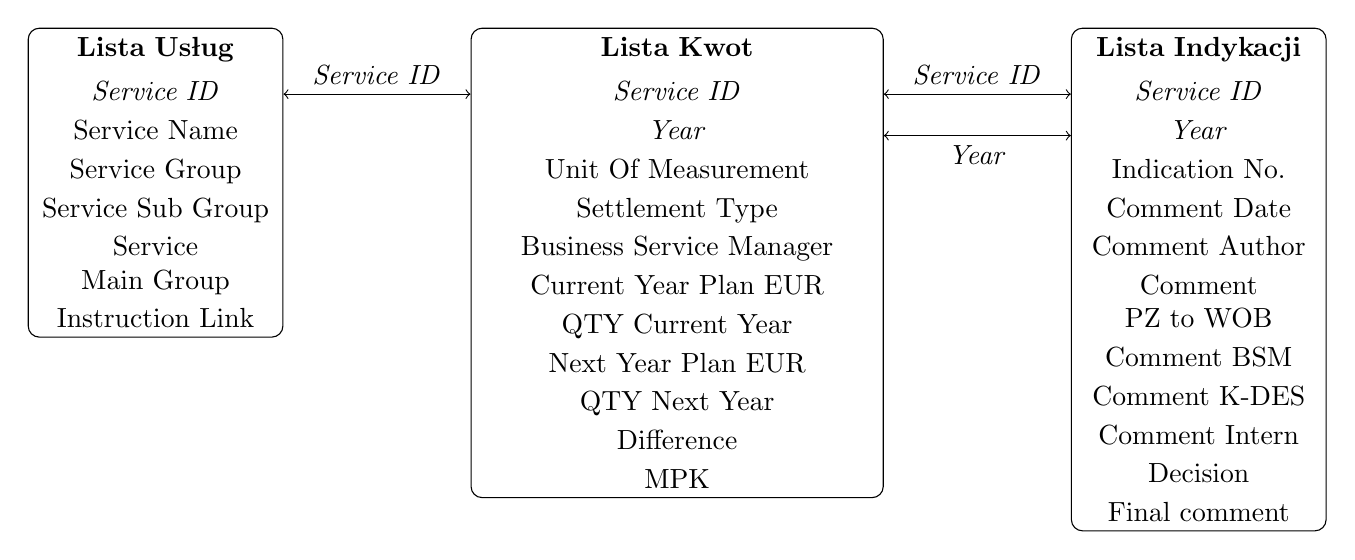
\begin{tikzpicture}

      \tikzstyle{ListBlock} = [
      rectangle,
      rounded corners,
      minimum width=3cm,
      minimum height=1cm,
      text centered,
      draw=black,
      fill=white,
      anchor=north
      ]

      \node (ListaUslug) [ListBlock, text width=3cm] at (0,0) {
        \textbf{Lista Usług}\\[4pt]
        \textit{Service ID}\\[2pt]
        Service Name\\[2pt]
        Service Group\\[2pt]
        Service Sub Group\\[2pt]
        Service Main Group\\[2pt]
        Instruction Link\\[2pt]
      };

      \node (ListaKwot) [ListBlock, text width=5cm]
      at ([xshift=5cm] ListaUslug.north east) {
        \textbf{Lista Kwot}\\[4pt]
        \textit{Service ID}\\[2pt]
        \textit{Year}\\[2pt]
        Unit Of Measurement\\[2pt]
        Settlement Type\\[2pt]
        Business Service Manager\\[2pt]
        Current Year Plan EUR\\[2pt]
        QTY Current Year\\[2pt]
        Next Year Plan EUR\\[2pt]
        QTY Next Year\\[2pt]
        Difference\\[2pt]
        MPK\\[2pt]
      };

      \node (ListaIndykacji) [ListBlock, text width=3cm]
      at ([xshift=4cm] ListaKwot.north east) {
        \textbf{Lista Indykacji}\\[4pt]
        \textit{Service ID}\\[2pt]
        \textit{Year}\\[2pt]
        Indication No.\\[2pt]
        Comment Date\\[2pt]
        Comment Author\\[2pt]
        Comment PZ to WOB\\[2pt]
        Comment BSM\\[2pt]
        Comment K-DES\\[2pt]
        Comment Intern\\[2pt]
        Decision\\[2pt]
        Final comment\\[2pt]
      };

      \draw [<->] ([yshift=-2em-4pt]ListaUslug.north east) -- node[anchor=south]{\textit{Service ID}} ([yshift=-2em-4pt]ListaKwot.north west);
      \draw [<->] ([yshift=-2em-4pt]ListaKwot.north east) -- node[anchor=south]{\textit{Service ID}} ([yshift=-2em-4pt]ListaIndykacji.north west);
      \draw [<->] ([yshift=-3.5em-4pt]ListaKwot.north east) -- node[anchor=north]{\textit{Year}} ([yshift=-3.5em-4pt]ListaIndykacji.north west);

    \end{tikzpicture}}
  \caption{Schemat relacji między listami.}
  \label{SchematList}
\end{figure}

Model danych przedstawiony na Rysunku \ref{SchematList} został zaprojektowany z uwzględnieniem następujących założeń:

\begin{itemize}
  \item \emph{Lista usług} pełni rolę centralnego rejestru serwisów, zawierając ich podstawową charakterystykę,
  \item \emph{Lista kwot} umożliwia śledzenie zmian w wymiarze finansowym na przestrzeni lat,
  \item \emph{Lista indykacji} przechowuje historię procesu decyzyjnego wraz z towarzyszącymi komentarzami i ustaleniami.
\end{itemize}




\subsection{Dodawanie informacji do bazy danych}
Po ustaleniu struktury danych wykorzystywanych przez system, należało określić w jaki sposób informacje z arkuszy kalkulacyjnych będą umieszczane w bazie danych.

Głównym problemem na tym etapie jest brak systematycznej organizacji danych zawartych w arkuszach programu Excel co prowadzi do braku kompatybilności z zaprojektowaną bazą danych. 
Zdecydowano się na utworzenie dedykowanego ekranu w aplikacji, który odpowiada za poprawne przetworzenie danych przy asyście użytkownika w celu uniknięcia błędów.

Pierwszym krokiem jest tymczasowe umieszczenie pliku Excel w folderze znajdujacym się we wspólnej przestrzeni roboczej programu Sharepoint. Dzięki temu, dokument jest dostępny dla innych systemów wykorzystanych do jego przetwarzania. Niestety pomimo możliwości otwarcia pliku przez inne systemy, dane w nim zawarte nie były widoczne. Jak się okazało, większość systemów jest w stanie odczytać informacje pogrupowane w \emph{tabele programu Excel}\footnote{W programie Excel tabelę trzeba osobno zadeklarować np. ręcznie zaznaczając zakres komórek a następnie wybierając opcję \emph{Narzędzia główne}$\to$\emph{Fromatuj jako tabelę}}.

Do rozwiązania tego problemu użyto skryptu pakietu Office, który działa wewnątrz arkusza a co za tym idzie ma bezpośredni dostęp do wszystkich informacji w nim zawartych. Skrypt ten oprócz tworzenia tabeli o dynamicznym rozmiarze, usuwa puste kolumny, które czasem były obecne wśród danych. Utworzony algorytm jest w stanie określić początek tabeli oraz jej wielkość zależną od liczby wierszy oraz kolumn, bez uwzględniania zbędnych informacji.

W celu przystosowania informacji z pliku do bazy danych, zdecydowano się na zastosowanie formularza do walidacji nazw kolumn. Formularz ten pobiera nazwy istniejących kolumn w zapisanym arkuszu i pozwala przypisać do nich nazwy z predefiniowanej listy zawierającej nagłówki znajdujące się w listach Sharepoint. Aktualne nazwy również pobierane są przy pomocy wcześniej opisanego skryptu.

Po usystematyzowaniu struktury użytkownik wybiera rok oraz numer indykacji, której dotyczy wgrywany arkusz. Następnie wszystkie informacje są przekazywane do \emph{flow} programu \emph{Power Automate}, które przypisuje je do odpowiednich listach bazy danych upewniając się, że nie powstają duplikaty.

Zdecydowano, że opisywany ekran będzie posiadał dodatkowy formularz odpowiedzialny za przypisywanie numerów \emph{MPK} dla nowych serwisów. Jest to bardzo ważne ponieważ numer ten okeśla, który obszar zajmuje się rozpatrzeniem usługi. W przypadku usług rozpatrywanych w latach poprzednich numer ten jest przepisywany aby ograniczyć liczbę wypełnianych danych. Oczywiście jest możliwość edycji istniejącego wcześniej numery w razie potrzeby. 
\subsection{Interfejs procesu decyzyjnego}
Interfejs obsługi procesu decyzyjnego został podzielony na dwa współpracujące ze sobą ekrany. Takie rozwiązanie pozwala na zachowanie przejrzystości prezentowanych informacji przy jednoczesnym zapewnieniu dostępu do wszystkich niezbędnych funkcjonalności.

\subsubsection{Ekran nawigacyjny}
Pierwszy ekran pełni rolę panelu nawigacyjnego, prezentującym kluczowe informacje dotyczące usługi:
\begin{itemize}
    \item Service Name -- nazwa serwisu,
    \item Service ID -- unikalny identyfikator usługi,
    \item MPK -- numer określający miejsce powstawania kosztów,
    \item Decision -- aktualny status decyzji.
\end{itemize}
Ponadto użytkownicy będą mieli możliwość filtrowania i wyszukiwania serwisów według następujących kryteriów:
\begin{itemize}
    \item wyszukiwanie serwisów względem ID,
    \item wyszukiwanie serwisów względem nazwy,
    \item filtrowanie według przypisanych numerów MPK,
    \item filtrowanie według statusu decyzji (\emph{Accepted}, \emph{Not Accepted}, \emph{No Status}).
\end{itemize}

\subsubsection{Ekran szczegółowy}
Po wybraniu serwisu z listy, użytkownik zostaje przekierowany do ekranu szczegółowego, który składa się z trzech głównych sekcji:
\begin{itemize}
    \item \textbf{Podgląd danych historycznych} -- prezentuje on zarówno ogólne informacje o serwisie zbierane na przestrzeni lat, jak i szczegóły dotyczące poszczególnych indykacji.
    \item \textbf{Formularz decyzyjny} -- zestaw pól do wprowadzenia informacji o bieżącej indykacji. Składają się na niego:
    \begin{itemize}
        \item rok (wartość domyślna: bieżący),
        \item numer indykacji (wartość domyślna: kolejny wolny numer),
        \item autor (wartość domyślna: zalogowany użytkownik),
        \item komentarze (wewnętrzny, BSM, K-DES),
        \item decyzja (wartość domyślna: poprzednia decyzja).
    \end{itemize}
    
\end{itemize}
\subsection{Generowanie raportu}
Ostatnim etapem cyklu obsługi procesu jest generowanie raportu, następnie przesyłanego do zakładu w Wolfsburgu w celu dalszych konsultacji. Raport jest tworzony na podstawie danych przechowywanych na listach SharePoint, co zapewnia spójność i aktualność informacji.

W dedykowanym oknie aplikacji użytkownik będzie mieć możliwość wyboru odpowiedniego roku oraz etapu (numer indykacji). Na podstawie tych informacji, system przetworzy podane kryteria, aby zgromadzić odpowiednie dane z różnych źródeł.

Kolekcja\footnote{Kolekcja (Power Apps) -- tymczasowy zbiór danych, przechowywanych lokalnie w aplikacji, umożliwiający zarządzanie rekordami podczas jej działania.} danych, utworzona na podstawie wybranych kryteriów, połączy dane z trzech list sharepointowych. Dzięki temu możliwe będzie skonsolidowanie danych w jedną, spójną strukturę, która zawierać będzie wszystkie niezbędne informacje do sporządzenia raportu. Utworzone zostaną mechanizmy wyszukiwania, które umożliwią powiązanie identyfikatorów usług z odpowiadającymi im rekordami, co zapewni integralność zgromadzonych danych.

Dodatkowo, w tym samym oknie aplikacji umożliwiony zostanie użytkownikowi dostęp do podglądu zgromadzonych danych w formie tabeli. Umożliwi to weryfikację poprawności i kompletności informacji przed wygenerowaniem raportu. Po zatwierdzeniu danych, system przekaże zgromadzoną kolekcję do Power Automate, gdzie zostaną one zmodyfikowane, w celu przygotowania raportu w odpowiednim formacie (tj. w formacie arkusza kalkulacyjnego \emph{Excel}) do odesłania.



\chapter{Implementacja}

W niniejszym rozdziale przedstawiono szczegóły techniczne zaimplementowanego rozwiązania. Omówione zostaną kluczowe aspekty
implementacyjne systemu, obejmujące wykorzystanie platformy Microsoft Power Platform - w szczególności
Power Apps do budowy interfejsu użytkownika oraz Power Automate do automatyzacji procesów biznesowych.
Ponadto, przedstawiona zostanie integracja z platformą SharePoint oraz implementacja skryptów
usprawniających pracę z pakietem Microsoft Office. Rozdział stanowi techniczne rozwinięcie przyjętych
założeń projektowych, prezentując metodykę realizacji poszczególnych komponentów systemu.

W ramach analizy technicznej zostaną szczegółowo omówione poszczególne komponenty systemu oraz sposób
ich integracji. Szczególna uwaga zostanie poświęcona mechanizmom przepływu danych, automatyzacji
procesów oraz implementacji logiki biznesowej w środowisku low-code. Istotnym elementem będzie również
prezentacja zastosowanych rozwiązań w zakresie bezpieczeństwa danych oraz optymalizacji wydajności
w kontekście platformy Microsoft 365.

\section{Ekran zapisu danych}

Zdecydowano, że pierwszym ekranem aplikacji będzie ekran zapisu danych. Decyzja ta wynika z faktu, że bez prztworzonych danych, utworzenie innych ekranów byłoby zdecydowanie trudniejsze. Ekran ten składa się z elementów, które zostaną omówione poniżej.

\subsection{Zapis pliku w chmurze}
Pierwszym krokiem jest zapis pliku w chmurze w celu udostepnienia go innym systemom. W tym celu wykorzystano kontrolkę\footnote{Kontrolka -- element służący do nawigacji, wyświetlania danych i obsługi aplikacji.} \emph{Attachment Control}. Pozwala ona na zapisanie pliku w pamięci aplikacji. Odbywa się to przez naciśnięcie przycisku \emph{"Dołącz plik"} lub przy użyciu mechaniki \emph{przeciągnij i upuść} (\english{Drag And Drop}). 

Aby przekazać plik oraz jego zawartość należy nacisnąć przycisk opisany jako \emph{Save attachments} znajdujący się pod wcześniej omawianym elementem. Naciścięcie go skutkuje wywołaniem szeregu funkcji opisanych we właściwości \emph{OnSelect}. W pierwszej kolejności sprawdzane jest, czy plik został załadowany. Jeśli tak, to wywoływany jest przepływ \emph{SaveFileAndRunScript}. Wynik przepływu jest zapisywany w zmiennej tablicowej, która w Power Apps określana jest jako \definicja{kolekcja}, o nazwie \emph{FlowOutput}. Po wykonaniu się przepływu, zapisane w kontrolce pliki są usuwane.

\subsubsection{Przepływ SaveFileAndRunScript}
Przepływ \emph{SaveFileAndRunScript} jest odpowiedzialny za zapisanie pliku w chmurze. W momencie wywołania przepływu plik jest przekazany jako parametr wejściowy. Przepływ ten składa się z kilku kroków, które zostaną omówione w kolejności ich wykonywania.

\begin{figure}[H]
    \centering
    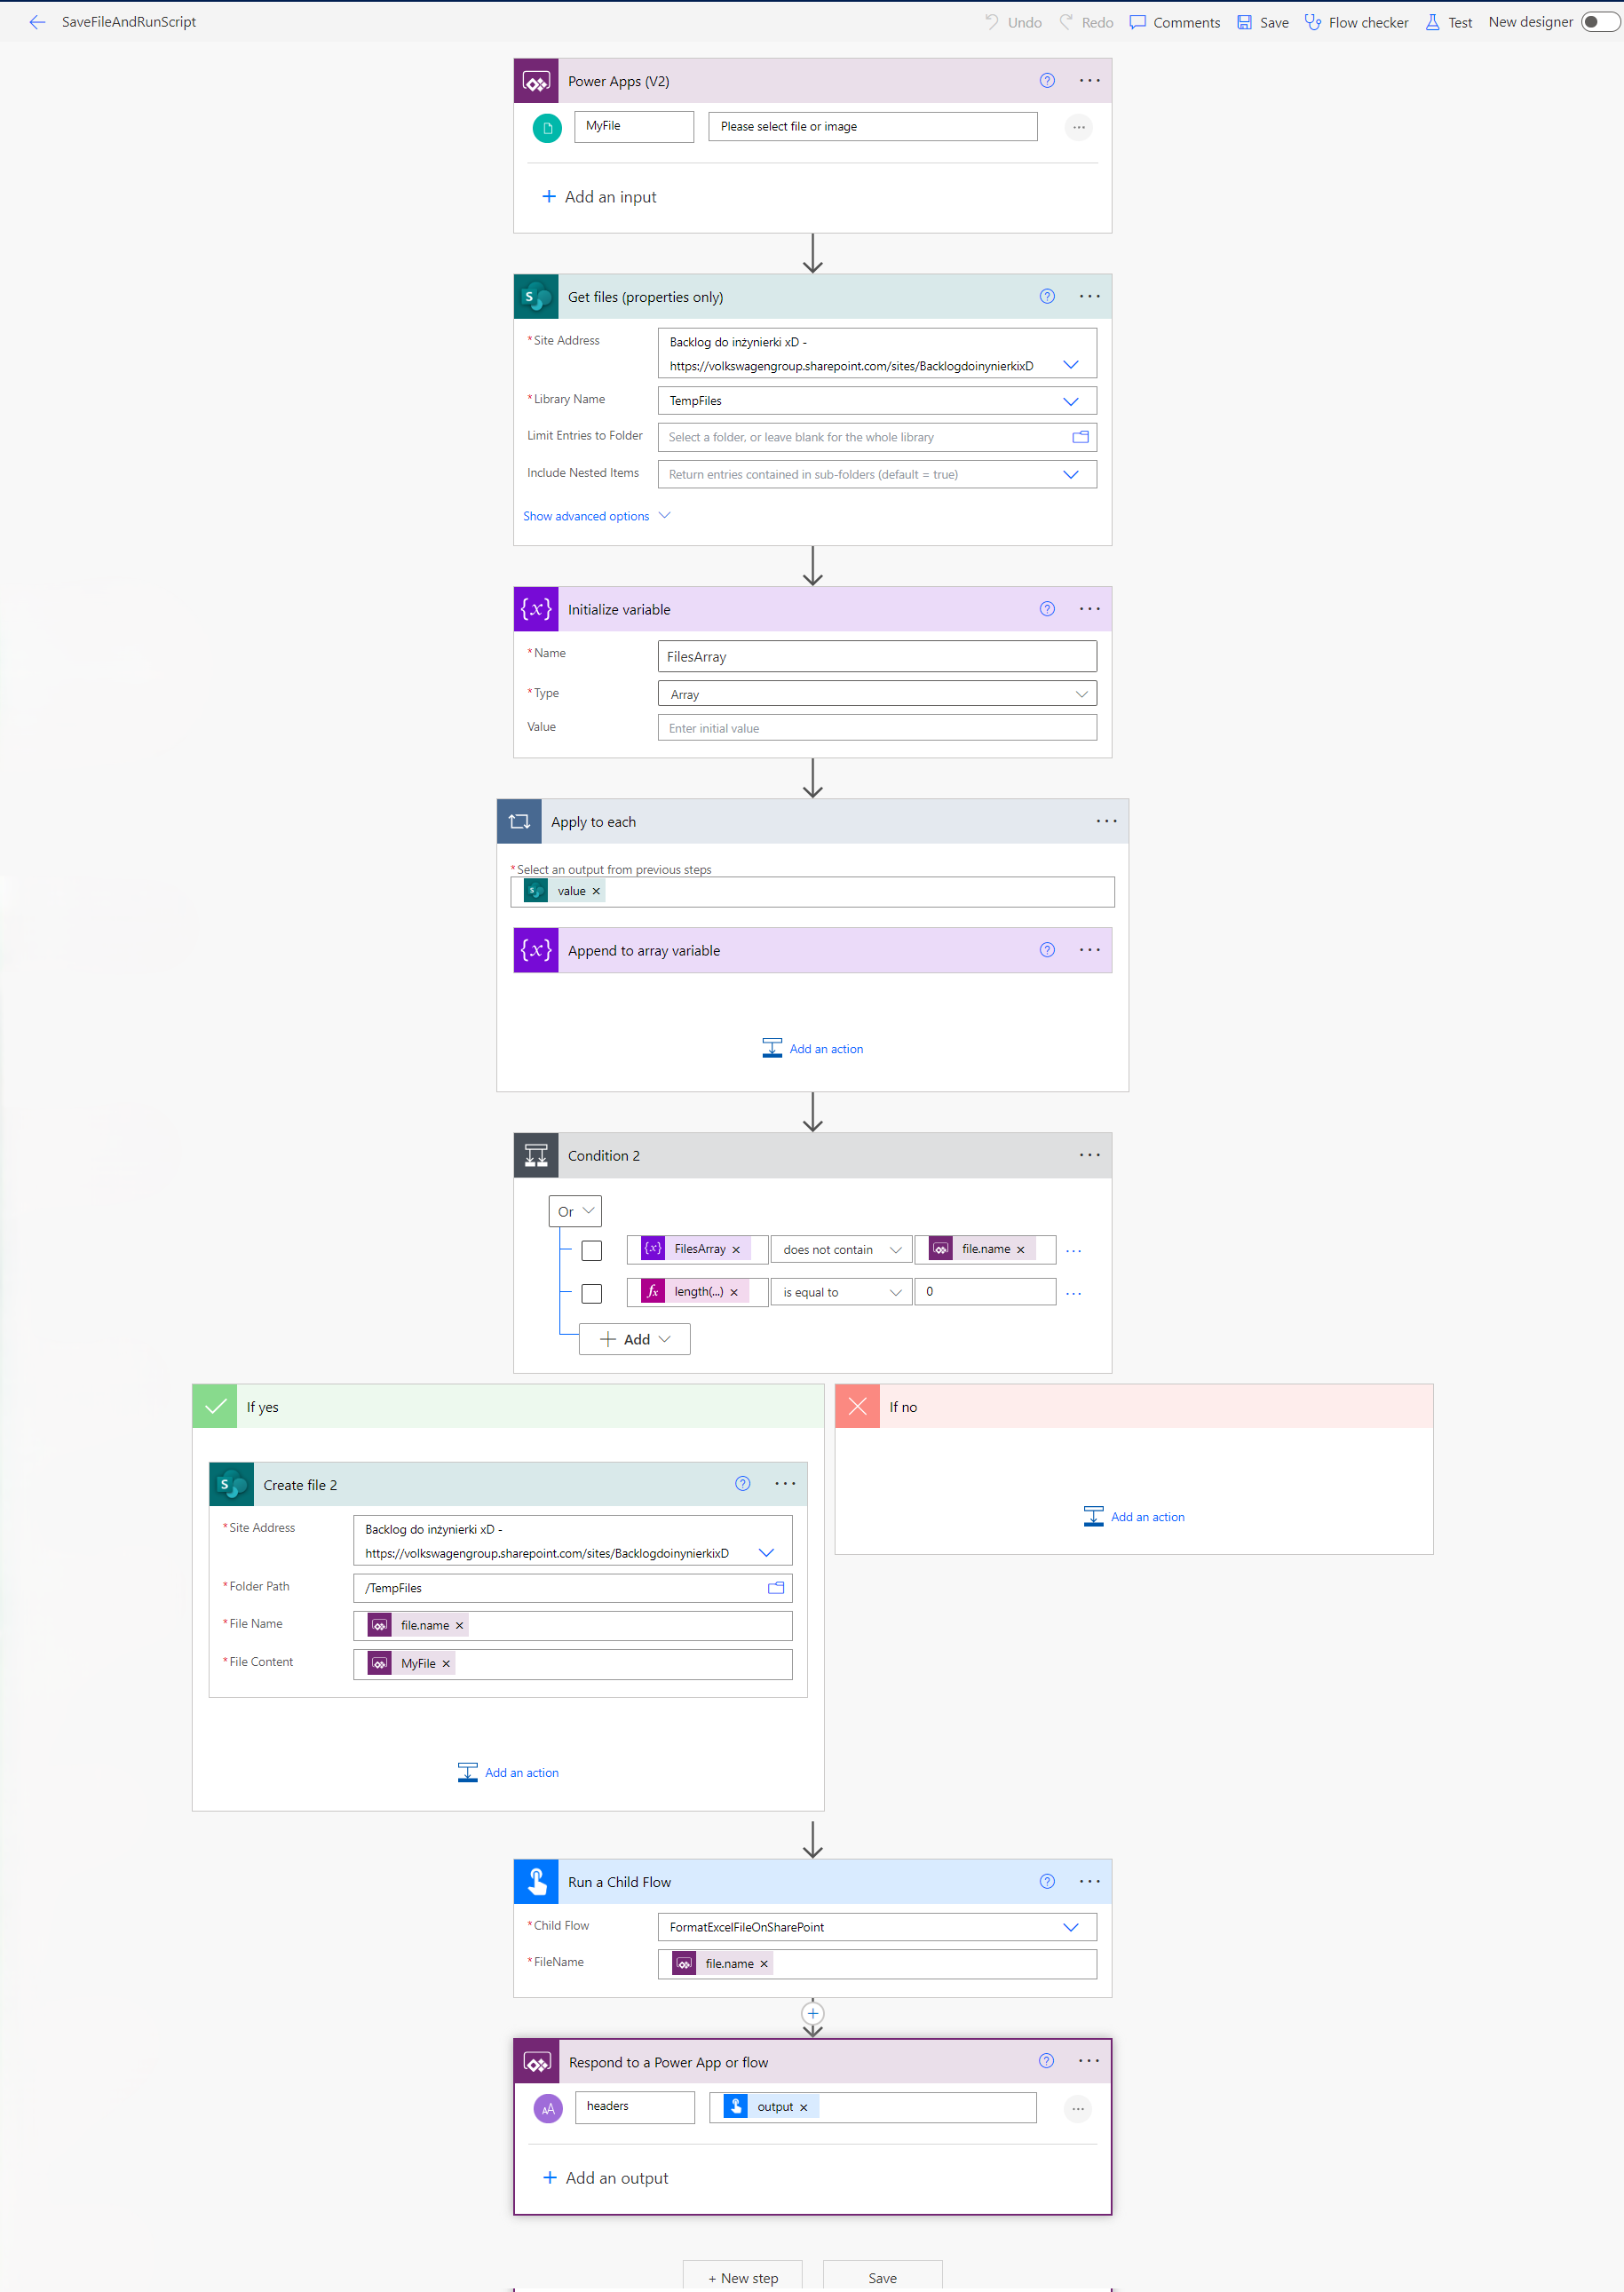
\includegraphics[width=0.85\textwidth]{figures/SaveFileAndRunScript.png}
    \caption{Widok przepływu SaveFileAndRunScript}
    \label{fig:savefileandrunscript}
\end{figure}

Rysunek \ref{fig:savefileandrunscript}, przedstawia widok przepływu \emph{SaveFileAndRunScript}. Przepływ ten składa się z następujących kroków:
\begin{enumerate}
    \item \textbf{Funkcja: Power Apps (V2)} \\
    Jest to element rozpoczynający przepływ, wywoływany bezpośrednio z aplikacji Power Apps. Parametrami wejściowymi są:
    \begin{itemize}
        \item nazwa pliku (\textit{File Name}),
        \item zawartość pliku (\textit{File Content}) w formacie binarnym.
    \end{itemize}

    \item \textbf{Sprawdzenie istniejących plików} \\
    Blok \textit{Get files (properties only)} pobiera listę wszystkich plików z wybranego folderu SharePoint wraz z ich metadanymi, takimi jak nazwa, ścieżka czy data modyfikacji. Pozwala to na sprawdzenie, czy plik o podanej nazwie już istnieje w bibliotece.

    \item \textbf{Warunek} \\
    Element \textit{Condition} sprawdza, czy istnieje plik o nazwie przekazanej w danych wejściowych. W zależności od wyniku:
    \begin{itemize}
        \item jeśli plik istnieje -- przepływ kończy działanie,
        \item jeśli plik nie istnieje -- kontynuuje proces zapisu.
    \end{itemize}

    \item \textbf{Utworzenie pliku} \\
    Blok \textit{Create file} tworzy nowy plik w SharePoint, wykorzystując parametry:
    \begin{itemize}
        \item adres witryny SharePoint,
        \item ścieżkę do folderu docelowego,
        \item nazwę pliku,
        \item zawartość pliku.
    \end{itemize}

    \item \textbf{Uruchomienie podprzepływu} \\
    Element \textit{Run a Child Flow} wywołuje skrypt Office Script, który:
    \begin{itemize}
        \item analizuje zapisany plik,
        \item sprawdza jego zawartość,
        \item formatuje dane według wymagań,
        \item zwraca wynik w formacie JSON.
    \end{itemize}

    \item \textbf{Odpowiedź do aplikacji} \\
    Blok \textit{Respond to Power Apps} kończy przepływ, zwracając do aplikacji dane w formacie JSON przetworzone przez wcześniej wspomniany skrypt Office Script.
\end{enumerate}

\subsection{Skrypt Office Script}
Po utworzeniu pliku w SharePoint, w ramach przepływu następuje jego przetworzenie przez skrypt Office Script. W tym przypadku skrypt ma za zadanie przeanalizować plik i dostosować go do wymagań systemu. Poniżej przedstawiono kroki działania skryptu:

\begin{enumerate}
    \item \textbf{Inicjalizacja i wybór arkusza}
    \begin{itemize}
        \item sprawdzenie wszystkich arkuszy w pliku Excel,
        \item wybór arkusza zawierającego dane,
        \item sprawdzenie i ewentualne usunięcie ochrony hasłem.
    \end{itemize}

    \item \textbf{Analiza danych}
    \begin{itemize}
        \item sprawdzenie czy dane są zorganizowane w tabeli,
        \item w przypadku braku tabeli -- utworzenie nowej,
        \item automatyczne uzupełnienie pustych miejsc w ważnych kolumnach.
    \end{itemize}

    \item \textbf{Dopasowanie nazw kolumn}
    \begin{itemize}
        \item porównanie istniejących nazw kolumn ze standardową listą,
        \item wykorzystanie algorytmu \emph{Jaro-Winkler} do oceny podobieństwa tekstu,
        \item automatyczne rozpoznawanie podobnych nazw (np. "Srv ID" jako "Service ID"),
        \item sugestia ręcznego wyboru przy zbyt małym podobieństwie (poniżej 90\%).
    \end{itemize}

    \item \textbf{Przekazanie wyników}
    \begin{itemize}
        \item zwrócenie oryginalnych nazw kolumn z pliku,
        \item zwrócenie dopasowanych standardowych nazw kolumn,
        \item w razie problemów - przekazanie odpowiednich komunikatów błędów.
    \end{itemize}
\end{enumerate}


\vspace{1cm}
Po zakończeniu działania skryptu Office Script i całego przepływu, przetworzony plik zostaje w pełni zapisany w bibliotece SharePoint. 
Rysunek \ref{fig:saveattachmentsform} przedstawia wspomnianą wcześniej kontrolkę \emph{Attachment Control}, przycisk \emph{Save attachments} oraz listę plików zapisanych w foldrze SharePoint.


\begin{figure}[h]
    \centering
    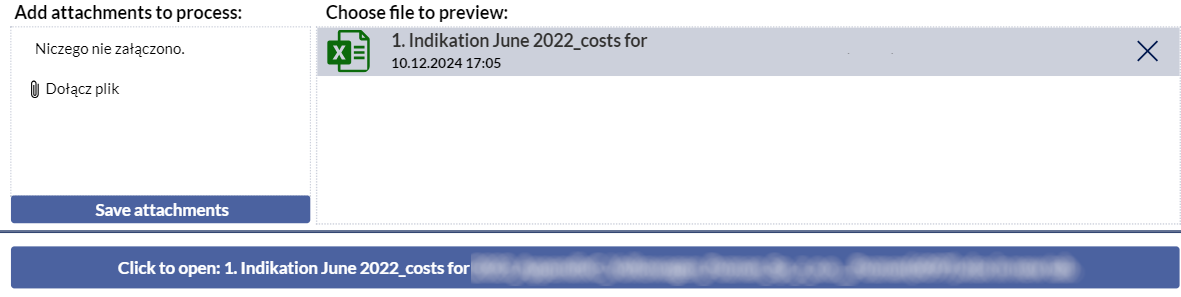
\includegraphics[width=\textwidth]
    {figures/SaveAttachmentsForm.png}
    \caption{Formularz zapisu pliku}    
    \label{fig:saveattachmentsform}
\end{figure}

Wybór elementu z listy \emph{Choose file to preview} umożliwia wskazanie pliku do dalszego przetwarzania. Selekcja pozycji z listy automatycznie inicjuje wykonanie opisanego wcześniej skryptu, którego celem jest pozyskanie aktualnego zestawu nagłówków. Należy podkreślić, że ten sam proces zachodzi również podczas inicjalizacji aplikacji. 
Funkcjonalność podglądu, zaimplementowana w postaci przycisku umiejscowionego poniżej głównych elementów sterujących, umożliwia otwarcie wybranego pliku w nowej karcie przeglądarki. Jest to szczególnie istotne w kontekście weryfikacji poprawności danych oraz walidacji struktury kolumn.

\chapter{Rozwinięcie}

Rozdziały dokumentujące pracę własną studenta: opisujące ideę, sposób lub metodę 
rozwiązania postawionego problemu oraz rozdziały opisujące techniczną stronę rozwiązania 
--- dokumentacja techniczna, przeprowadzone testy, badania i uzyskane wyniki. 

Praca musi zawierać elementy pracy własnej autora adekwatne do jego wiedzy praktycznej uzyskanej w
okresie studiów. Za pracę własną autora można uznać np.: stworzenie aplikacji informatycznej lub jej
fragmentu, zaproponowanie algorytmu rozwiązania problemu szczegółowego, przedstawienie projektu 
np.~systemu informatycznego lub sieci komputerowej, analizę i ocenę nowych technologii lub rozwiązań
informatycznych wykorzystywanych w przedsiębiorstwach, itp. 

Autor powinien zadbać o właściwą dokumentację pracy własnej obejmującą specyfikację założeń i 
sposób realizacji poszczególnych zadań
wraz z ich oceną i opisem napotkanych problemów. W przypadku prac o charakterze 
projektowo-implementacyjnym, ta część pracy jest zastępowana dokumentacją techniczną i użytkową systemu. 

W pracy \textbf{nie należy zamieszczać całego kodu źródłowego} opracowanych programów. Kod źródłowy napisanych
programów, wszelkie oprogramowanie wytworzone i wykorzystane w pracy, wyniki przeprowadzonych
eksperymentów powinny być przekazane promotorowi oraz wgrane wraz z pracą do systemu informatycznego uczelni.

\section*{Styl tekstu}

Należy\footnote{Uwagi o stylu pochodzą częściowo ze stron prof. Macieja Drozdowskiego.} \cite{Drozdowski2006} 
stosować formę bezosobową, tj.~\emph{w pracy rozważono ......, 
w ramach pracy zaprojektowano ....}, a nie: \emph{w pracy rozważyłem, w ramach pracy zaprojektowałem}. 
Odwołania do wcześniejszych fragmentów tekstu powinny mieć następującą postać: ,,Jak wspomniano wcześniej, ....'', 
,,Jak wykazano powyżej ....''. Należy unikać długich zdań. 

Niedopuszczalne są zwroty używane w języku potocznym. W pracy należy używać terminologii technicznej, która ma sprecyzowaną treść i znaczenie. 

Niedopuszczalne jest pisanie pracy metodą \emph{copy-paste}, bo jest to plagiat i dowód intelektualnej indolencji autora.
Dane zagadnienie należy opisać własnymi słowami. Zawsze trzeba powołać się na zewnętrzne źródła. 



\chapter{Zakończenie}

Zakończenie pracy zwane również Uwagami końcowymi lub Podsumowaniem powinno zawierać ustosunkowanie
się autora do zadań wskazanych we wstępie do pracy, a w szczególności do celu i zakresu pracy oraz
porównanie ich z faktycznymi wynikami pracy. Podejście takie umożliwia jasne określenie stopnia
realizacji założonych celów oraz zwrócenie uwagi na wyniki osiągnięte przez autora w ramach jego
samodzielnej pracy.

Integralną częścią pracy są również dodatki, aneksy i załączniki zawierające stworzone w ramach pracy programy, aplikacje i projekty.



%--------------------------------------
% Literatura
%--------------------------------------

\bibliographystyle{plain}{\raggedright\sloppy\small\bibliography{bibliografia}}

%--------------------------------------
% Dodatki
%--------------------------------------

\cleardoublepage\appendix%
\newpage

\chapter{Składanie dokumentu w systemie \LaTeX}

W tym rozdziale znajduje się
garść informacji o tym, jak poprawnie składać tekst pracy w systemie \LaTeX{} wraz z 
przykładami, które mają służyć do przeklejania do własnych dokumentów.

\section{Struktura dokumentu}
\chaptermark{Tytuł rozdziału, jeśli pełen się nie mieści\ldots{}}{}

Praca składa się z rozdziałów (\texttt{chapter}) i podrozdziałów (\texttt{section}).
Ewentualnie można również rozdziały zagnieżdzać (\texttt{subsection}, \texttt{subsubsection}),
jednak nie powinno się wykraczać poza drugi poziom hierarchii (czyli \texttt{subsubsection}).

\section{Akapity i znaki specjalne}

Akapity rozdziela się od siebie przynajmniej jedną pustą linią. Podstawowe
instrukcje, które się przydają to \emph{wyróżnienie pewnych słów}. Można również
stosować \textbf{styl pogrubiony}, choć nie jest to generalnie zalecane.

Należy pamiętać o zasadach polskiej interpunkcji i ortografii. Po spójnikach 
jednoliterowych warto wstawić znak tyldy ($\sim$), który jest tak zwaną
,,twardą spacją'' i powoduje, że wyrazy nią połączone nie będą rozdzielane
na dwie linie tekstu.

Polskie znaki interpunkcyjne różnią się nieco od angielskich: to jest ,,polski'', a to jest
``angielski''. W kodzie źródłowym tego tekstu będzie widać różnicę.

Proszę również zwrócić uwagę na znak myślnika, który może być pauzą ,,---'' lub
półpauzą: ,,--''. Należy stosować je konsekwentnie. Do łączenia wyrazów używamy
zwykłego ,,-'' (\emph{północno-wschodni}), do myślników --- pauzy lub półpauzy.
Inne zasady interpunkcji i typografii można znaleźć w słownikach.

\section{Wypunktowania}

Wypunktowanie z cyframi:
\begin{enumerate}
    \item to jest punkt,
    \item i to jest punkt,
    \item a to jest ostatni punkt.
\end{enumerate}

\noindent
Po wypunktowaniach czasem nie warto wstawiać wcięcia akapitowego. Wtedy przydatne jest
polecenie \texttt{noindent}. Wypunktowanie z kropkami (tzw.~\emph{bullet list}) wygląda tak:
\begin{itemize}
    \item to jest punkt,
    \item i to jest punkt,
    \item a to jest ostatni punkt.
\end{itemize}

\noindent
Wypunktowania opisowe właściwie niewiele się różnią:
\begin{description}
    \item[elementA] to jest opis,
    \item[elementB] i to jest opis,
    \item[elementC] a to jest ostatni opis.
\end{description}


\section{Polecenia pakietu \texttt{ppcreefthesis}}

Parę poleceń zostało zdefiniowanych aby uspójnić styl pracy. Są one przedstawione poniżej
(oczywiście nie trzeba się do nich stosować).

\paragraph{Makra zdefiniowane dla języka angielskiego.} Są nimi: \texttt{termdef} oraz \texttt{acronym}.
Przykłady poniżej obrazują ich przewidywane użycie w tekście.
\begin{center}\footnotesize%
\begin{tabular}{l >{\rightskip\fill}p{12cm}}
\toprule
źródło   & \texttt{we call this a $\backslash$termdef\{Database Management System\} ($\backslash$acronym\{DBMS\})} \\ \cmidrule(lr){2-2}
docelowo & we call this a \termdef{Database Management System} (\acronym{DBMS}) \\ 
\bottomrule
\end{tabular}
\end{center}

\paragraph{Makra zdefiniowane dla języka polskiego.} Podobnie jak dla języka angielskiego zdefiniowano
odpowiedniki polskie: \texttt{defini\-cja}, \texttt{akronim} oraz \texttt{english} dla tłumaczeń angielskich
terminów. Przykłady poniżej obrazują ich przewidywane użycie w tekście.
\begin{center}\footnotesize%
\begin{tabular}{l >{\rightskip\fill}p{12cm}}
\toprule
źródło   & \texttt{nazywamy go $\backslash$definicja\{systemem zarządzania bazą danych\} ($\backslash$akronim\{DBMS\}, $\backslash$english\{Database Management System\})} \\ \cmidrule(lr){2-2}
docelowo & nazywamy go \definicja{systemem zarządzania bazą danych} (\akronim{DBMS}, \english{Database Management System}) \\ \bottomrule
\end{tabular}
\end{center}


\section{Rysunki}

Wszystkie rysunki (w tym również diagramy, szkice i inne) osadzamy w środowisku 
\texttt{figure} i umieszczamy podpis \emph{pod} rysunkiem, w formie elementu \texttt{caption}. Rysunki powinny
zostać umieszczone u góry strony (osadzone bezpośrednio w treści strony zwykle utrudniają czytanie tekstu).
Rysunek~\ref{rys:plama} zawiera przykład pełnego osadzenia rysunku na stronie.

\begin{figure}[t] % możliwe opcje to 't' - top, 'b' - bottom, 'h' - 'here', ale zaleca się 't'
\centering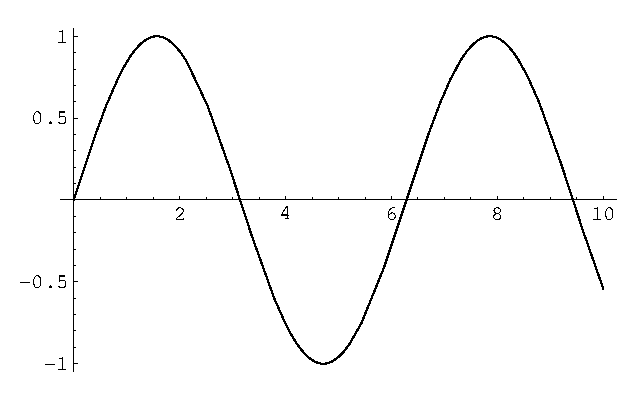
\includegraphics[width=5cm]{figures/mathematica}
\caption{Wykres.}\label{rys:plama}
\end{figure}

\begin{figure}[t]
\centering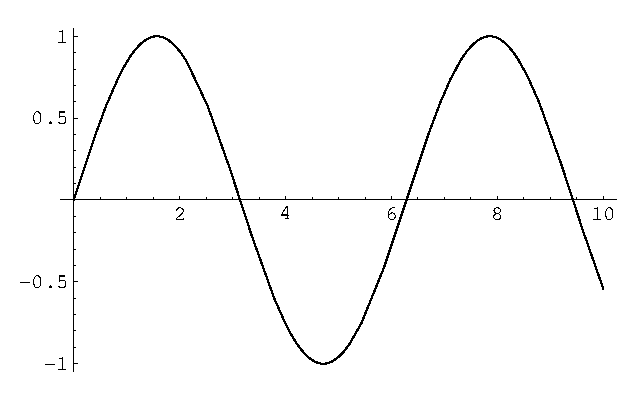
\includegraphics[width=\textwidth]{figures/mathematica}
\caption{Ten sam wykres ale na szerokość tekstu.} \label{rys:plama2}
\end{figure}


\subsection{Tablice}

Tablice to piękna rzecz, choć akurat ich umiejętne tworzenie w \LaTeX{}u nie jest łatwe. 
Jeśli tablica jest skomplikowana, to można ją na przykład wykonać w programie
OpenOffice, a następnie wyeksportować jako plik \akronim{PDF}. W każdym przypadku tablice wstawia się podobnie
jak rysunki, tylko że w środowisko \texttt{table}. Tradycja typograficzna sugeruje umieszczenie opisu tablicy, a więc
elementu \texttt{caption} ponad jej treścią (inaczej niż przy rysunkach).  

Tablica~\ref{tab:tabela} pokazuje pełen przykład.

\begin{table}[ht]
\caption{Przykładowa tabela. Styl opisu jest zgodny z rysunkami.}\label{tab:tabela}
\centering\footnotesize%
\begin{tabular}{l c}
\toprule
artykuł & cena [zł] \\
\midrule
bułka   & $0,4$ \\
masło   & $2,5$ \\
\bottomrule
\end{tabular}
\end{table}


\subsection{Przydatne uwagi}

\begin{itemize}
\item Znakiem myślnika jest w LaTeXu dywiz pełen (---) albo półpauza (--), przykład:
  A niech to jasna cholera --- wrzasnąłem.

\item Połączenie między wyrazami to zwykły myślnik, przykład:   północno-zachodni

\item Sprawdź ostrzeżenia o 'overfull' i 'underful' boxes. Niektóre z nich można zignorować (spójrz
  na wynik formatowania), niektóre trzeba poprawić; czasem przeformułować zdanie.

\item Przypisy stawia się wewnątrz zdań lub za kropką, przykład:
  Footnote is added after a comma.\footnote{Here is a footnote.}

\item Nie używaj przypisów zbyt często. Zobacz, czy nie lepiej będzie zintegrować przypis z tekstem.

\item Tytuły tabel, rysunków powinny kończyć się kropką.

\item Nie używaj modyfikatora [h] (here) do rysunków i tabel. Rysunki i tabele powinny być
  justowane do góry strony lub na stronie osobnej.

\item Wyróżnienie w tekście to polecenie \emph{wyraz}, należy unikać \textbf{czcionki pogrubionej} i \underline{podkreślenia} (które wystają wizualnie z tekstu i rozpraszają).

\item Nazwy plików, katalogów, ścieżek, zmiennych środowiskowych, klas i metod formatujemy poleceniem
  \texttt{plik\_o\_pewnej\_nazwie}.

\item Po ostatniej zmianie do treści, sprawdź i przenieś wiszące spójniki wstawiając przed nie znak
  tyldy (twardej spacji), przykład:
  Ala i~kotek nie lubią mleczka, a~Stasiu lubi.
  
\item Za i.e. (id est) i e.g. (exempli gratia) stawia się zwyczajowo przecinek w typografii amerykańskiej.

\item Przed i za pełną pauza nie ma zwyczajowo spacji w typografii amerykańskiej, przykład:
  Darn, this looks good---said Mary.

\item Zamykający cudzysłów oraz footnote wychodzą za ostatni znak interpunkcji w typografii 
  amerykańskiej, przykłady:
  It can be called a ``curiosity,'' but it's actually normal.
  Footnote is added after a comma.\footnote{Here is a footnote.}

\item Odwołania do tabel i rysunków zawsze z wielkiej litery, przykład:
  In Figure~\ref{rys:plama} we illustrated XXX and in Table~\ref{tab:tabela} we show detailed data.
  
\end{itemize}


\section{Literatura i materiały dodatkowe}

Materiałów jest mnóstwo. Oto parę z nich:
\begin{itemize}
    \item \emph{The Not So Short Introduction\ldots}, która posiada również tłumaczenie 
    w języku polskim.\\
    \url{http://www.ctan.org/tex-archive/info/lshort/english/lshort.pdf}

    \item Klasy stylu \texttt{memoir} posiadają bardzo wiele informacji o składzie tekstów
    anglosaskich oraz sposoby dostosowania \LaTeX{}a do własnych potrzeb.\\
    \url{http://www.ctan.org/tex-archive/macros/latex/contrib/memoir/memman.pdf}
    
    \item Nasza grupa dyskusyjna i repozytorium Git są również dobrym miejscem aby zapytać
    (lub sprawdzić czy pytanie nie zostało już zadane).\\
    \url{https://github.com/politechnika/put-latex}

    \item Dla łaknących więcej wiedzy o systemie LaTeX podstawowym źródłem informacji
    jest książka Lamporta~\cite{Lamport1985}. Prawdziwy \emph{hardcore} to oczywiście
    \emph{The \TeX{}book} profesora Knutha~\cite{Knuth1986}.
\end{itemize}



%--------------------------------------
% Informacja o prawach autorskich
%--------------------------------------

\ppcolophon

\end{document}
